
%%%%%%%%%%%%%%%%%%%%%%%%%%%%%%%%%%%%%%%%%%%%%%%%%%%%%%%%%%%%%%%%%%% 
%                                                                 %
%                           INTRODUCTION                          %
%                                                                 %
%%%%%%%%%%%%%%%%%%%%%%%%%%%%%%%%%%%%%%%%%%%%%%%%%%%%%%%%%%%%%%%%%%% 
 
\chapter{INTRODUCTION}
\label{chapter:intro}

% magical first sentence
% explain like you would to your parents/non-technological people
% - explain how keyframe animation currently works
% explain in more technical terms what this means
% - problems with current techniques
% - what can be done (auto animation)
% - overview of controllers
% - overview of the technique
% explain contributions
% - what is the contribution of this technique
% - Unity3D -> what am I getting from outside sources
% - what am I making myself

Animations of human characters are used heavily in video games, movies, and other fields.  Creation of such animations is largely done by hand by artists using keyframing.  In a keyframe animation, certain ``key'' parts of the animated sequence are specified, with the remaining frames filled in, or ``tweened'' using an automated interpolation method or manual frame addition.  For 2D animation, this occurs as a series of images which are played back in order to produce the animation.  In 3D, keyframe animations are performed on a 3D model.

% figure of sprite animation frames

3D models are described as a mesh, a collection of primitive polygons (i.e. quadrilaterals or triangles) which are stored as vertices.  This mesh describes what is drawn, including any texture, color, and other material information.  Along with the mesh, a skeleton, or rig, is stored.  The rig describes a heirarchical structure of bones and accompanying joints.  Each vertex is given a series of weights describing the impact each joint has on its transformation.  This allows many vertices, and therefore many polygons, to be transformed at once in organized groups, simplifying the problem of animating the model to a matter of transforming the skeleton in the desired manner.  To animate this 3D model, an artist specifies keyframes of the animation by positioning the skeleton.  The stored keyframes, instead of an image, are the transformations of each joint at this frame in the animation, which a rendering or game engine can interpolate between to produce the final animation.

Specifying these animation frames is work intensive, taking up significant time and resources to produce for a single character.  Recent work in animation generation seeks to automate this process, replacing the manual process with a procedural one.  Physics based simulations can be used to produce controllers for the skeleton, determining joint positions and rotations for keyframes automatically.  Not only does this reduce the effort involved in the creation process, but this also provides a basis for dynamic interaction between a character's animation and the environment, which is not possible with manual keyframe animations.

% figure of current keyframe animation process in maya
% accompanying video for presentation
% accompanying figure/video of the resulting animation in 3d

%sean's stuff below here

\begin{figure}[htp] \centering
    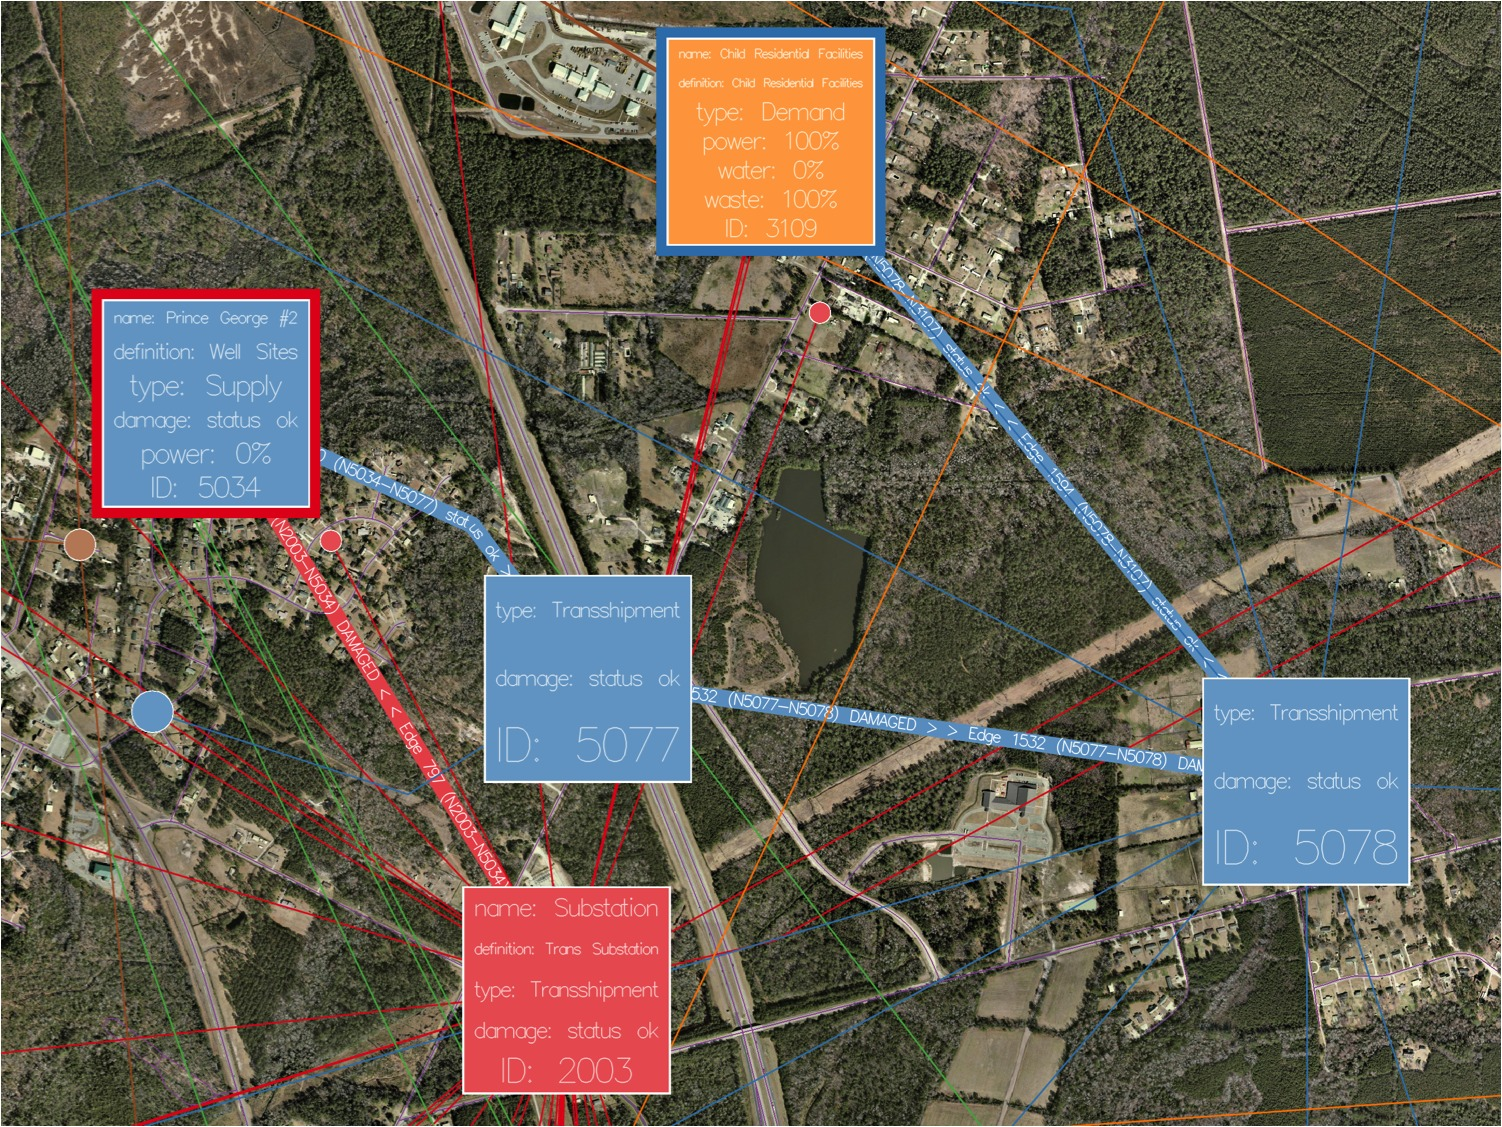
\includegraphics[width=0.8\linewidth]{img/mapview_example.jpg}
    \caption[Example Infrastructure Visualization]{This example screenshot shows an example scenario of a residential node lacking water,
    by following the network back to the supply node, we can deduce that the overall problem is twofold, a lack of power
    to the water supply node and a damaged water pipe - both must be addressed to restore water to the demand node.}
    \label{fig:mapview_example}
\end{figure}

When expanded, each node provides its id and name. If it is either a supply or transshipment node, it has a
corresponding status which indicates if it is currently supplying its resource to its edges. If a node requires a particular resource to function, it shows the current ratio of the supply and demand for that resource as a percentage. Edges show their current status: {\tt damaged} or {\tt status OK} as well as their ids and two corresponding node ids. If either a node or an edge is damaged, it is unable to transmit its resource.

When interacting with the system, users can toggle different parts of the display to simplify the data being presented. The underlying road network and satellite images can be turned off, as well as the nodes and edges of a particular resource. Users can also increase the level of detail of the application, effectively zooming in and out on the satellite images. This allows the users to see the a more detailed view of the satellite images and also reduces the number of graph elements on the screen. 

This entire application is designed to work with a system developed by Tyler Sammann and Chris Stuetzle, and which allows multiple users to interact with a system with mouse cursors and laser pointers \cite{Sammann2013}. These various input devices are generalized as cursors which have a generalized set of gestures, allowing for collaboration on a single screen between multiple users. In the context of the viewer application, this functionality allows the users to expand and
collapse the different graph elements, navigate to different areas of the map, change the global level of detail, and toggle the visibility of different elements as described above.

Systems that use multiple cursors are designed to foster collaborative problem solving and data exploration. Having multiple people interact with a system all at once allows people do explore different areas of the data set at the same time where normally a single person would control what everyone using the system sees. By having users work on a single shared screen instead of multiple displays, each individual user can more easily see what other people are looking at or
modifying.

Previous demonstrations of this application revealed that the current functionality was lacking a number of features that would allow for greater information visibility. Essentially, users are unable to view a particular region in a higher level of detail without possibly disturbing what the other users are viewing. Figure~\ref{fig:example_problem} presents an example of this issue.

\begin{figure}[htp] \centering
    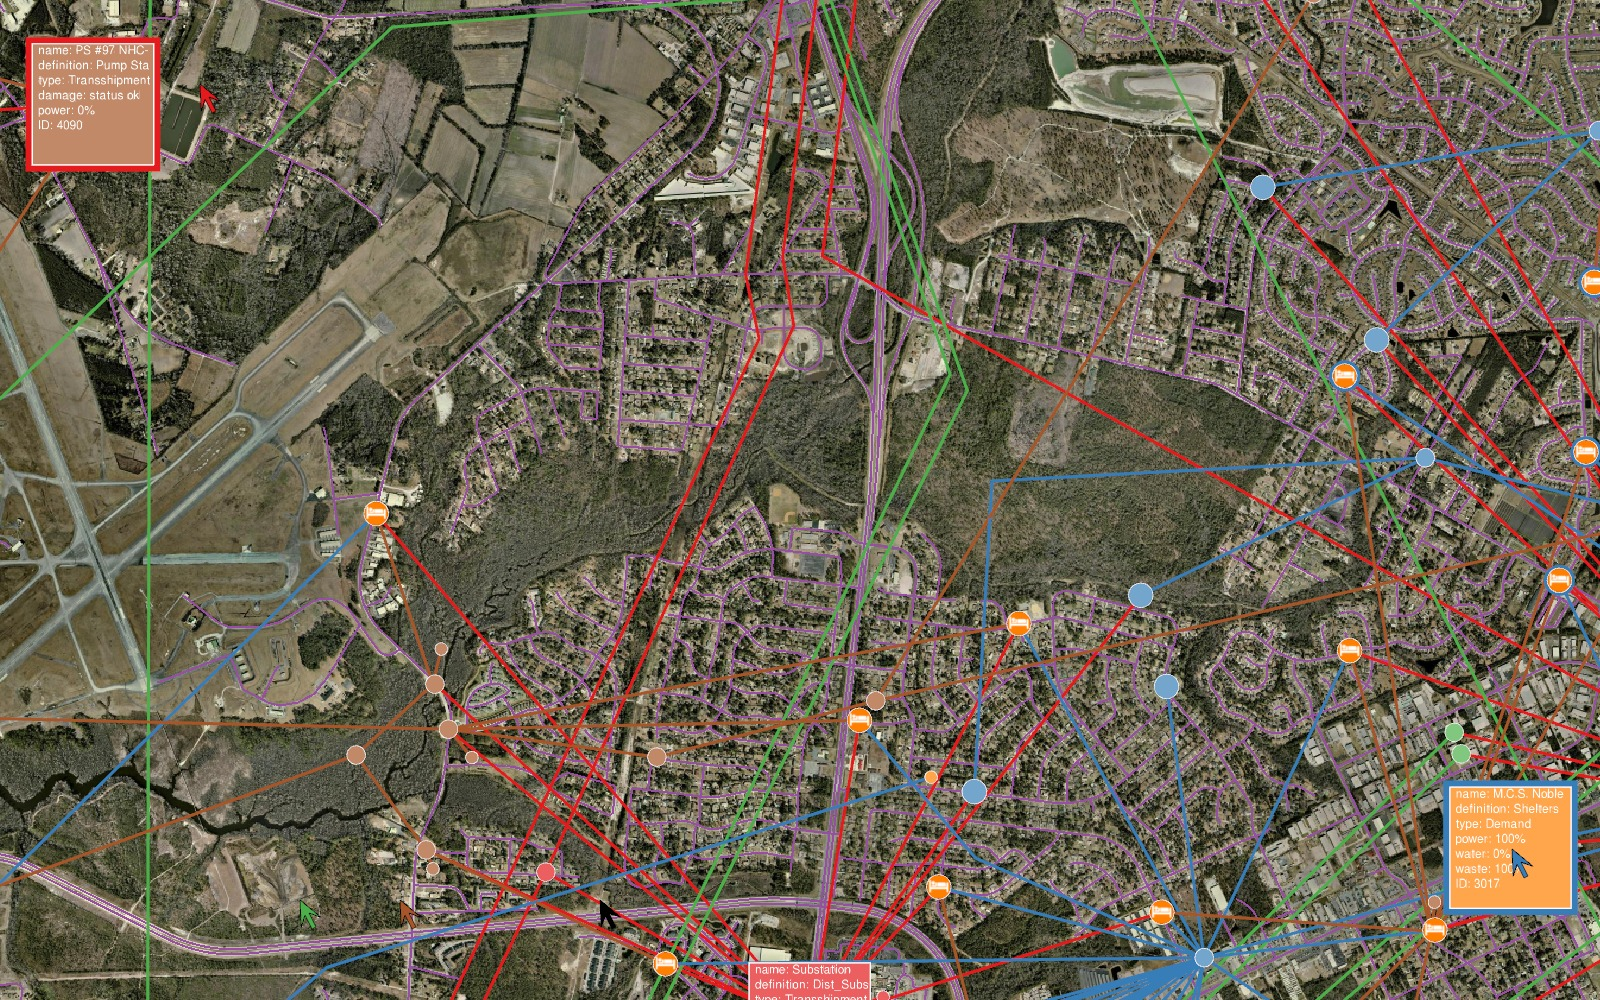
\includegraphics[width=150mm]{img/global_zoom_problem.jpg}
    \caption[Loss of Context]{This diagram shows a screenshot with two cursors in different regions of the application. The red arrow cursor is in the top left corner and the blue arrow cursor is in the bottom right corner. If either cursor performs a global zoom on their location to get more detail, the other cursor is unable to view their data.}
    \label{fig:example_problem}
\end{figure}

A system allowing for multiple areas of magnification when integrated with the previously mentioned multi-cursors could be useful in other contexts. If examining any sort of large graph based data set, being able to view different focal areas in higher detail would allow users to navigate data sets easier while still viewing the overall graph structure.

\section{Focus Plus Context}
\label{section:intro_fac}
Overview plus detail, zooming, and focus plus context are all methods within information visualization for displaying data. They each seek to present varying levels of data in a format that facilitates understanding. Overview plus detail visualizations are similar to physical maps of cities. The overall view of a city is shown on the big map, but a higher detail region of the city is shown in a separate, enclosed area (Figure~\ref{fig:louisiana}). This sort of visualization is easy to create, and is most
common for static media, as certain areas inherently require more detail than others when dealing with static data. Being able to interactively change the level of detail is the principle behind zooming visualizations (Figure~\ref{fig:google_maps}). This method is well suited for a single user looking to view different levels of detail at different points in time. It is also relatively easy to implement and does not cause distortions in the data being displayed. Focus plus context systems are useful for systems
where a user needs both a local and global view at the same time. Some loss of data can occur in these visualizations, but by using a single screen, the user does not need to mentally combine the data of a overview plus detail visualization. The first two formats separate data in two
different ways: overview plus detail interfaces separate data spatially, while zooming separates data temporally. Focus plus context uses a visual effect to display continuous information on a single screen \cite{Cockburn2008}. 

\begin{figure}[htp] \centering
    \includegraphics[width=0.8\linewidth]{img/1853_Louisiana.jpg}
    \caption[Overview Plus Detail]{This old map of Louisiana from 1853 showing a detailed view of a streets of New Orleans is an example of an overview plus detail visualization \cite{Mitchell1853}.}
    \label{fig:louisiana}
\end{figure}

\begin{figure}[htp] \centering
    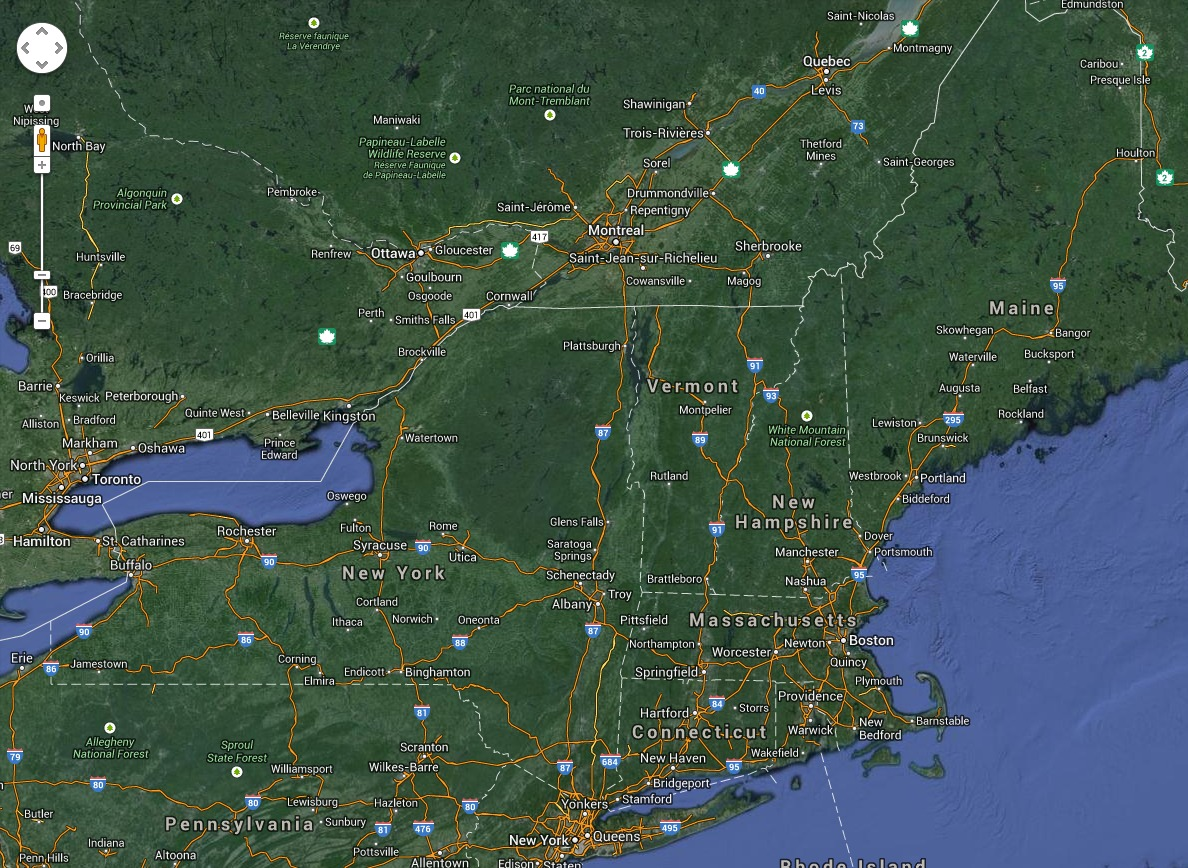
\includegraphics[width=0.8\linewidth]{img/zoom_interface.jpg}
    \caption[Zooming Interface]{An image of a common zooming interface for map data, Google Maps \cite{google_maps}.}
    \label{fig:google_maps}
\end{figure}

The goal of focus plus context interfaces is to reduce the cognitive load of managing multiple different views 
of a single system. Theoretically, this would improve user performance with regards to understanding and 
utilizing the data being presented. The foundation for the focus plus context interfaces was established by Furnas in 1986
\cite{Furnas1986}. He described a ``generalized fisheye view'' formula is described which 
calculates a user's ``degree of interest'' (\emph{DOI}) \cite{Furnas1986} (Equation~\ref{eq:furnas_doi}). The degree of interest, given a data element \emph{x} and focus \emph{y}, is the \emph{a priori interest} (API) in the data element minus the distance between the data element and the focus, \emph{D}.  The term fisheye in photography refers to a strong visual distortion which has an extremely wide angle. This photographic technique allows for more detail
in the resulting image by introducing distortion. The ``generalized fisheye view'' states that objects closer to the focal point are more important than ones further away, paralleling the fact that in a fisheye visualization, objects close to the focal point are less distorted.

\begin{equation}
    \label{eq:furnas_doi} 
    DOI(x, y) = API(x) - D(x,y)
\end{equation}

Focus plus context systems often perform some sort of distortion to present the data. Further work by Furnas within focus plus context systems highlighted the crucial fact that distortion based visualizations achieve a seamless display by requiring the user to understand that data is being modified in some manner \cite{Furnas2006}. All such distortions perform some sort of filtering of the data, as the distortion functions are presented on media with finite limitations. As information
gets further distorted, it is essentially filtered out, as it can no longer be discerned by the users. Distortion causes geometric distortion among the data, altering the positions and shapes, while maintaining topological continuity. This property is potentially desirable, as our application features satellite images, which should remain topologically continuous \cite{Furnas2006}. By remaining topologically continuous, users would still be able to discern the
relative distance between any two points on the map, as there are no regions of completely missing data.

Due to the nature of the data that we are working with, techniques that introduce some sort of distortion to achieve a focus plus context visualization are particularly relevant to the work presented in this thesis. Leung and Apperley provide an overview of such techniques\cite{Leung1994}. Among the relevant applications are the Polyfocal Display \cite{Kadmon1978}, the Perspective Wall \cite{Mackinlay1991}, and the Graphical Fisheye View \cite{Sarkar1992}. These techniques are further explored in
Chapter~\ref{chapter:previous_work}. Leung and Apperley classifies such techniques as magnification functions. The different functions can be further divided into techniques that have continuous magnification functions and those with noncontinuous piecewise functions. The different functions are unified into a single metaphor of a stretchable sheet on a rigid frame. By increasing the amount of data displayed in a single area, i.e. ``stretching'' the sheet to display information, other areas must ``shrink'' and display less data. The overall distortion effect that is then displayed is a result of the stretching and shrinking of the display.
This stretchable rubber metaphor holds up even for views with multiple foci, though it is paramount that the balance between magnification and demagnification is maintained, otherwise the ``frame'' of the sheet would be deformed. At the core of \cite{Leung1994} is the idea that all of these distortion techniques are similar, and are purely dependent upon a single magnification function. We will expand upon this idea of creating a magnification function for our visualization later on in Chapter~\ref{chapter:magnification}.

\section{Thesis Outline and Contributions}
\label{section:intro_outline}
As mentioned earlier, the first draft of the infrastructure visualization program has the ability to
recognize simultaneous input from multiple keyboards, computer mice, and lasers by individual participants, but only supported zooming on a global scale. This loss of information when performing a global zoom is a major hindrance to a system which should be used by multiple people at the same time. If diagnosing a central problem for discrete graph elements in different geographic regions, trying to get more information about the area around a node is impossible with the
current model without disrupting the other users. The main goals in designing this new system were to provide users the ability to view different regions of data at a variable level of detail without altering a majority of the
global context. Because this visualization may be viewed by people who are not directly interacting with the system, solutions that cause too much loss of global context should be avoided. If we change the global context, we run into the same issue of obscuring other regions of high importance. 

The first step in creating a solution which met our needs was the design and implementation of a proof-of-concept system. An investigation of previous methods of focus plus context visualizations was performed to formulate the design behind our solution, detailed in Chapter~\ref{chapter:previous_work}. The concepts learned from this system were then applied to the pre-existing application. The visualization required many changes to allow for the new feature to be implemented and a large bulk of time was spent on upgrading to modern OpenGL to also improve performance; these changes are detailed in Chapter~\ref{chapter:visualization}. Two separate magnification functions were created to affect both the satellite imagery and the
graph network. These functions, described in Chapter~\ref{chapter:magnification}, cause the graph elements to stay in the same geographic location, and are easily adjustable for different parameters. The speed of the new system with regards to rendering and performing the magnification functions was measured and recorded in Chapter~\ref{chapter:results}. Chapter~\ref{chapter:results} also includes an informal survey of untrained user responses was carried out to gauge the basic
usability of the new magnification system. Finally, further improvements and changes to the system are discussed in Chapter~\ref{chapter:future_work}.
